%% ma: L11-B29-0001
%% lop: 11
%% chuong: 8
%% bai: 29
%% dang: 11.29.1
%% loai: TLN
%% muc: VDC
%% dap_an: "267"
%% nguon: "Ảnh giáo viên gửi 24/10/2026 (M06): Kỳ thi thử đợt IV, Thi thử TN THPT 2027 (Biên soạn: Aimbet), Phần 3 Câu 5"
%% kien_thuc: "Lớp 10 Bài 23-24 (quy tắc đếm, hoán vị), Bài 26 (xác suất cổ điển); Lớp 11 Bài 6 (cấp số cộng), Bài 29 (công thức cộng xác suất cho hai biến cố)"
%% ghi_chu: "Bổ sung '(mỗi khu đất xây một tòa nhà)' cho rõ. Đáp án tự giải, kiểm bằng duyệt hết 8! cách xếp bằng Python"
%% trang_thai: chinh-thuc
\begin{ex}
Trong một dự án bất động sản, người ta dự định xây $8$ tòa nhà có số tầng lần lượt là $2$, $3$, $4$, $5$, $7$, $8$, $9$, $10$ trên $4$ khu đất nằm tại phân khu phía Tây $A$, $B$, $C$, $D$ và $4$ khu đất nằm tại phân khu phía Đông $E$, $F$, $G$, $H$ (mỗi khu đất xây một tòa nhà). Ban quản lí của dự án quy định rằng hai tòa nhà được xây trên hai khu đất $C$, $F$ có số tầng nhiều nhất lần lượt tại phân khu phía Tây, phân khu phía Đông và tại ít nhất một phân khu, có $3$ tòa nhà có số tầng tạo thành một cấp số cộng. Gọi xác suất để cách xây $8$ tòa nhà thỏa mãn quy định là $\dfrac mn$ với $\dfrac mn$ là phân số tối giản và $m,n$ là các số nguyên dương. Giá trị của biểu thức $n-m$ bằng bao nhiêu?
\begin{center}
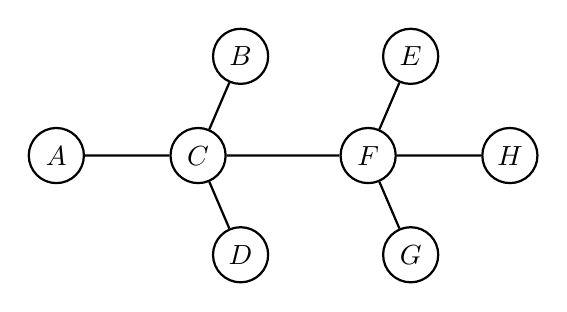
\begin{tikzpicture}[scale=.9,o/.style={circle,draw,thick,minimum size=7mm,inner sep=0pt}]
  \node[o] (C) at (0,0) {$C$}; \node[o] (F) at (2.4,0) {$F$};
  \node[o] (A) at (-2,0) {$A$}; \node[o] (H) at (4.4,0) {$H$};
  \node[o] (B) at (.6,1.4) {$B$}; \node[o] (D) at (.6,-1.4) {$D$};
  \node[o] (E) at (3,1.4) {$E$}; \node[o] (G) at (3,-1.4) {$G$};
  \draw[thick] (A)--(C)--(F)--(H) (B)--(C)--(D) (E)--(F)--(G);
\end{tikzpicture}
\end{center}
\shortans{267}
\loigiai{Không gian mẫu: $8!=40\,320$ cách. Đếm cách chọn tập $W$ gồm $4$ số cho phía Tây (phía Đông là $8$ số còn lại); với mỗi cách chọn, tòa cao nhất mỗi bên đặt cố định tại $C$, $F$, ba tòa còn lại mỗi bên xếp $3!$ cách, nên mỗi tập cho $3!\cdot3!=36$ cách.
Gọi $T_1$: phía Tây có $3$ số lập cấp số cộng, $T_2$: phía Đông có. Liệt kê $\mathrm C_8^4=70$ tập $W$: số tập thỏa $T_1$ là $35$, thỏa $T_2$ là $35$, thỏa cả hai là $18$; thỏa $T_1$ hoặc $T_2$: $35+35-18=52$ tập.
Số cách thuận lợi $52\cdot36=1\,872$. $P=\dfrac{1\,872}{40\,320}=\dfrac{13}{280}$, $n-m=267$.}
\end{ex}
